\chapter{Umsetzung}
\label{chap:implementation}

Nachdem die Ziele der angestrebten TypeScript-Migration charakterisiert und die Anforderungen an den geplanten Transpiler ausgeführt wurden, soll im Folgenden der Entwurf und die Details der entsprechend gewählten Implementierung ausgeführt werden. In Abschnitt~\ref{subsec:js-transpilers} wurden bereits die verbreitetsten Werkzeuge zur Transformation von JavaScript-Quelltexten ausführlich vorgestellt und verglichen. Auf Basis dieser Gegenüberstellung wurde schließlich Babel~\autocite{BABEL} als Grundlage der vorliegenden Umsetzung des Transpilers von Flow nach TypeScript gewählt.

\section{Software-Architektur}

\subsection{Konzeptioneller Aufbau des Transpilers}

Mit der Entscheidung den Übersetzer als Babel-Plugin zu implementieren, ist dessen Grundarchitektur bereits in Teilen festgelegt, da alle Plugins die vorgegebenen Programmschnittstellen von Babel erfüllen müssen\footnote{Vgl. Abschnitt~\ref{subsection:babel-plugins}.}. Bevor auf Details der Umsetzung eingegangen wird, soll zunächst der grundsätzliche Aufbau des Programms skizziert werden. Abbildung~\ref{fig:architecture-overview} verschafft einen Überblick über die verschiedenen Komponenten des Systems und deren Beziehung zueinander.

Die Architektur gliedert sich in zwei Teile: Ein Kommandozeilenprogramm stellt die Benutzerschnittstelle dar, welche verschiedene Optionen bereit stellt und die Eingabe-Verzeichnisse bzw. -Dateien als Argument entgegen nimmt. Die zweite Komponente ist ein Babel-Plugin, welches die Transpilierung des Flow-Codes nach TypeScript realisiert. Das Kommandozeilenprogramm liest sukzessive alle Eingabeverzeichnisse bzw. -dateien ein und startet intern die Transpilierung des Quelltexts mittels Babel, indem das vorliegende Plugin eingesetzt wird. Anschließend kann der generierte TypeScript-Code in Dateien bzw. auf die Standardausgabe geschrieben werden.

Das Plugin setzt sich aus verschiedenen Unterkomponenten zusammen: Auf oberster Ebene befinden sich Besucher-Funktionen, welche die gewünschten Pfade des abstrakten Syntaxbaums während dessen Traversierung adressieren. Diese Routinen rufen Konverter"=Funktionen auf, welche die Übersetzung der Flow-Knoten in ihr entsprechendes TypeScript-Pendant umsetzen.
% TODO: ACHJA? wirklich?
Bei der Verarbeitung der Knoten kommt es dabei auch zu rekursiven Aufrufen der Konverter. In einigen Fällen werden weiterhin Methoden zur Optimierung des Transformationsresultats ausgeführt.

\begin{figure}[tbp]
  \centering
  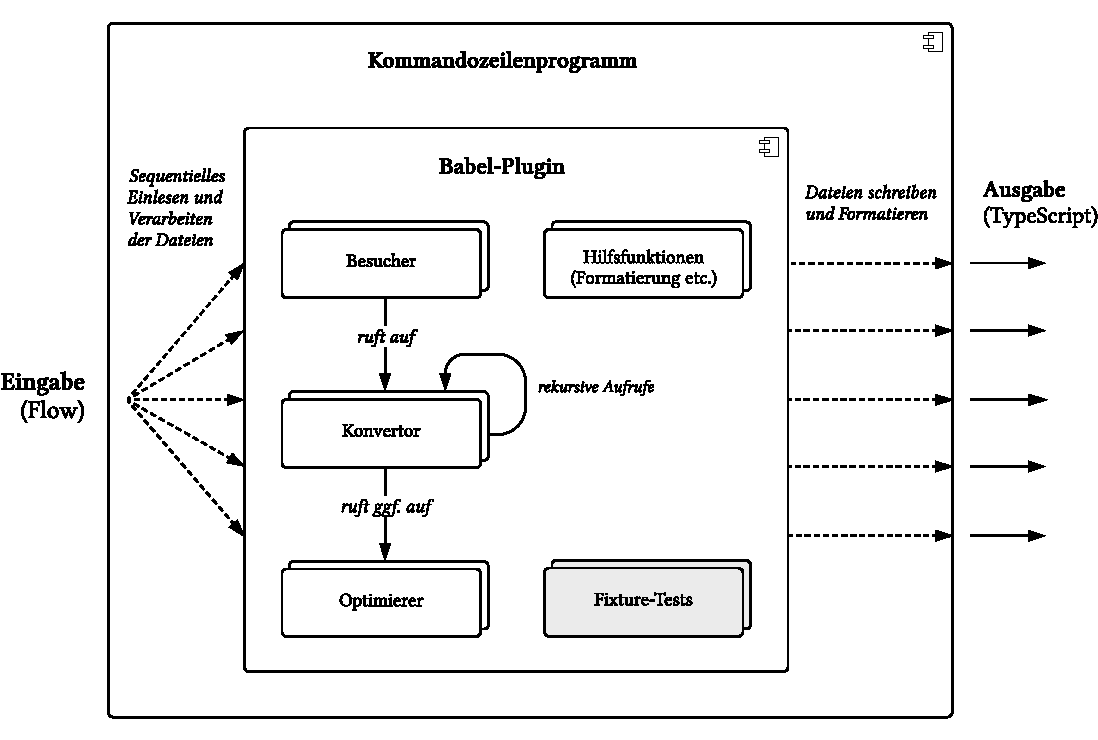
\includegraphics[width=0.92\textwidth]{src/4_Umsetzung/img/architecture-overview.pdf}
	\caption{Überblick über Komponenten des Transpilers}
	\label{fig:architecture-overview}
\end{figure}

\section{Entwicklungsprozess}

\subsection{Eingesetzte Technologien}

TypeScript alter und so

\subsection{Testgetriebene Entwicklung}

Die korrekte Übersetzung der Flow-Typen ist die wichtigste Anforderung an den Transpiler\footnote{Vgl. Anforderung \ref{subsection:requirement:correct-translation}.}. Essentiell ist daher die Bereitstellung zuverlässiger Testmechanismen, um Regressionen während der Entwicklungphase frühzeitig festzustellen. Zur Gewährleistung dieser Anforderung wurde der Ansatz der \enquote{testgetriebenen Entwicklung}\footnote{engl. \textit{Test-driven development (TDD).}} gewählt, um die korrekte Funktionalität und Wechselwirkung aller Bestandteile des Transpilers kontinuierlich zu überprüfen. Die testgetriebene Entwicklung hat ihren Ursprung im Vorgehensmodell \enquote{Extreme Programming}~\autocite{JEFFRIES:EXTREME_PROGRAMMING} aus der Software-Entwicklung und sieht im Gegensatz zu klassischen, seriellen Vorgehensweisen wie dem Wasserfall-Modell vor, dass alle Testfälle eines Features bereits \emph{vor} dessen Umsetzung geschrieben werden müssen~\autocite{KENT:EXTREME_PROGRAMMING}. Die Vorteile dieser Methodik ist die Sicherstellung einer hohen Testabdeckung und die Erzielung einer Implementierung, welche die Anforderungen \emph{vollständig} erfüllt, sofern die Testfälle sorgfältig spezifiziert wurden.



% Verlagerung des Fokus auf die korrekte Erfüllung der Software-Anforderungen, indem diese .

% Hierdurch wird sicher gestellt, dass der Programmierer sich \emph{zuerst} Gedanken über die konkrete Eingabe und erwartete Ausgabe einer Funktion machen muss und erst danach mit der Umsetzung beginnt.

% da auf diese Weise sichergestellt wird, dass eine hohe Testabdeckung der Transformationsroutinen besteht.

% Irgendwo sollte wohl geschrieben werden, dass TypeScript, TDD usw. verwendet wurde, um das Plugin zu bauen\dots

\section{Implementierung als Babel-Plugin}
  \subsection{Überblick}

  Abbildung~\ref{fig:activity-diagram-plugin} veranschaulicht den detaillierten Aufbau des Plugins anhand eines Aktivitätsdiagramms\footnote{Aktivitätsdiagramme entstammen der Modellierungssprache \textit{Unified Modeling Language} (UML)~\autocite{OMG:UML} und veranschaulichen den Ablauf einer Aktivität innerhalb eines Software-Systems.}. Zu Beginn wird das Plugin wie im Grundlagenteil in Quelltext~\ref{code:babel-plugin-definition} bereits exemplarisch gezeigt initialisiert, d.~h. es wird eine Abbildung der Flow-Knotentypen auf Besucher-Funktionen definiert. Weiterhin werden die Abhängigkeiten des Plugins spezifiziert. Bei diesen Abhängigkeiten handelt es sich um Babel-Plugins, die das Parsen der Syntax von Flow, JSX und vorgeschlagener\footnote{Erweiterungen der ECMAScript-Spezifikation } ECMAScript-Spracherweiterungen wie beispielsweise Klassenattribute~\autocite{} ermöglichen.

  \begin{figure}[tbp]
    \centering
    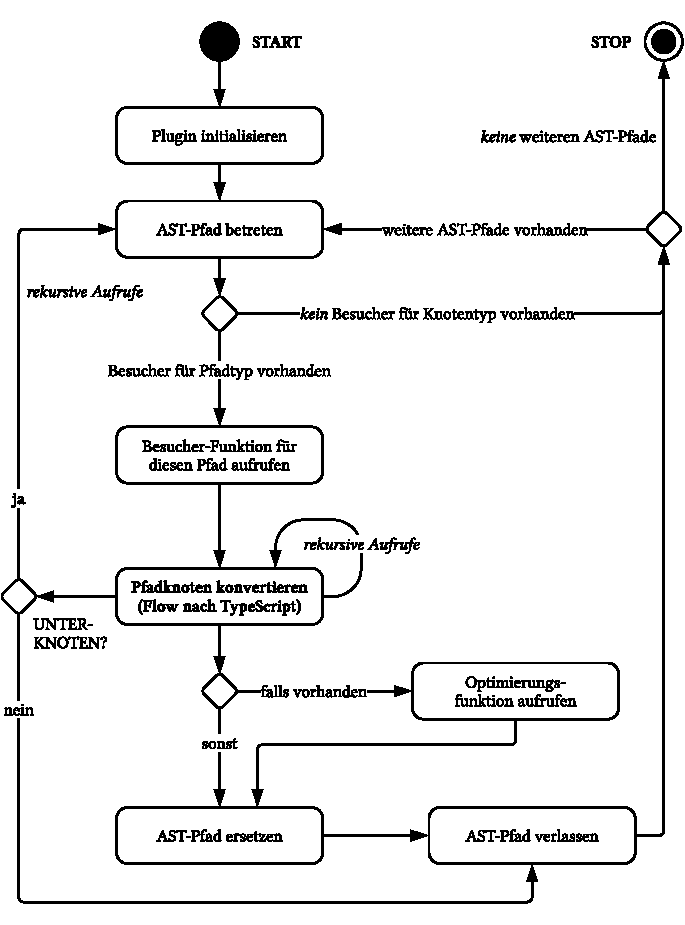
\includegraphics[width=0.85\textwidth]{src/4_Umsetzung/img/activity-diagram-plugin.pdf}
    \captionsetup{justification=centering}
    \caption{Aktivitätsdiagramm des Transpilers (Babel-Plugin).}
    \label{fig:activity-diagram-plugin}
  \end{figure}

  \subsection{Transpilierung der Basistypen}
  \subsection{Transpilierung der Hilfstypen}
  \subsection{Transpilierung der Deklarationen}

  \subsection{Weitere Optimierungen}
    \subsubsection{Übersetzung gängiger Typimporte}
    \subsubsection{Konvertierung von Class Decorators}

  Mapping der Importe (verschiedene Typnamen in Flow und TS), Umwandlung der Decorators usw.

\section{Erweiterung als Kommandozeilenprogramm}

Aufgrund der in Abschnitt~\ref{subsection:requirement:batch-processing} dargelegten Anforderung, dass der Transpiler in der Lage sein muss gesamte Projektverzeichnisse zu verarbeiten, ist eine Erweiterung als Kommandozeilenprogramm naheliegend. Hierdurch können beliebige Dateien und Verzeichnisse eingelesen und übersetzt werden.

% Dieses nimmt einzelne Eingabedateien oder -verzeichnisse als Argument entgegen und besitzt weiterhin verschiedene Optionen, um den Transpilierungsvorgang

Abbildung~\ref{fig:activity-diagram-cli} auf Seite~\pageref{fig:activity-diagram-cli} zeigt das Aktivitätsdiagramm der Anwendung.
% Dieses stellt lediglich eine schmale Ummantelung des Babel-Plugins dar
% Dieses bietet diverse Optionen, welche dem Benutzer ermöglichen die Transpilierung

\begin{figure}[tbp]
  \centering
  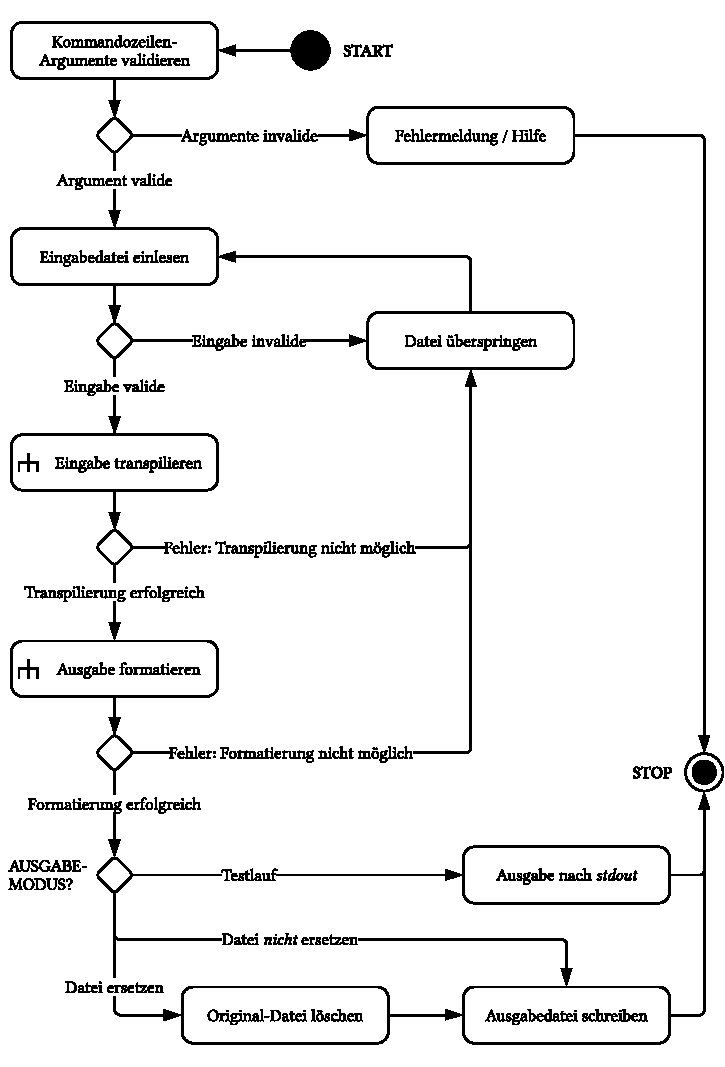
\includegraphics[width=0.85\textwidth]{src/4_Umsetzung/img/activity-diagram-cli.pdf}
	\caption[Aktivitätsdiagramm des Kommandozeilenprogramms]{Aktivitätsdiagramm des Kommandozeilenprogramms. Vgl. eingebettete Diagramme~\ref{fig:activity-diagram-plugin} \enquote{Eingabe transpilieren} und~\ref{fig:activity-diagram-formatting} \enquote{Ausgabe formatieren}.}
	\label{fig:activity-diagram-cli}
\end{figure}

\section{Formatierung des Ausgabequelltexts}

Eine weitere Problematik, die sich während der Entwicklung des Transpilers gezeigt hat, ist die Formatierung des resultierenden Ausgabecodes. Da Babel auf Grundlage eines \emph{abstrakten} Syntaxbaums arbeitet, liegt nach der Transformation des Programms keinerlei Information mehr über die ursprüngliche Formatierung des Codes vor\footnote{Diese Information wäre innerhalb eines konkreten Syntaxbaums TODO}. Die Einrückung und die Position der Leerzeichen und -zeilen gehen somit in der generierten Ausgabe verloren. Es hat sich weiterhin herausgestellt, dass auch die Position der Kommentare nach Anwendung des Babel-Plugins nicht präzise beibehalten wird. Die Leerzeilen und Kommentare tragen

Zur Erfüllung der in Abschnitt~\ref{subsection:requirement:format} ausgeführten Anforderung, dass die Formatierung so

\begin{figure}[htbp]
  \centering
  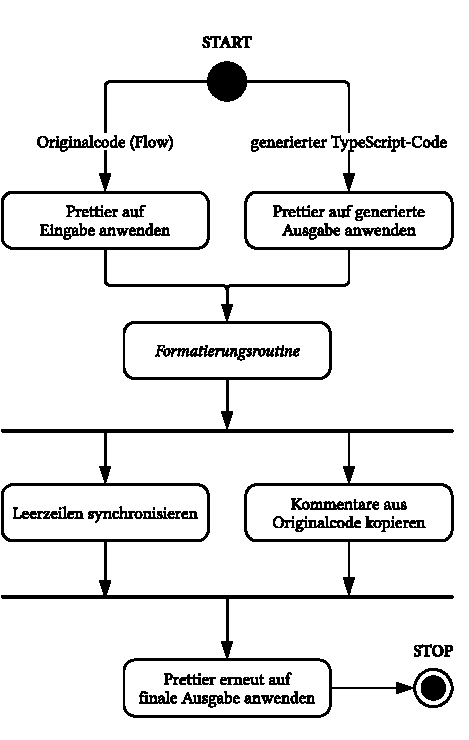
\includegraphics[width=0.6\textwidth]{src/4_Umsetzung/img/activity-diagram-formatting.pdf}
  \captionsetup{justification=centering}
	\caption[Aktivitätsdiagramm der Formatierung des Ausgabecodes]{Aktivitätsdiagramm der Formatierung des generierten Ausgabecodes.}
	\label{fig:activity-diagram-formatting}
\end{figure}

Prettier, synchronisieren der Leerzeilen und Kommentare beschreiben usw.
